\chapter{Część praktyczna}
\label{cha:praktyka}

\section{Prosta sieć konwolucyjna}
\subsection{Struktura}
\begin{verbatim}
Model:
_________________________________________________________________
Layer (type)                 Output Shape              Param #   
=================================================================
conv2d_1 (Conv2D)            (None, 118, 158, 32)      896       
_________________________________________________________________
max_pooling2d_1 (MaxPooling2 (None, 59, 79, 32)        0         
_________________________________________________________________
dropout_1 (Dropout)          (None, 59, 79, 32)        0         0.2
_________________________________________________________________
conv2d_2 (Conv2D)            (None, 57, 77, 64)        18496     
_________________________________________________________________
max_pooling2d_2 (MaxPooling2 (None, 28, 38, 64)        0         
_________________________________________________________________
dropout_2 (Dropout)          (None, 28, 38, 64)        0         0.2
_________________________________________________________________
conv2d_3 (Conv2D)            (None, 26, 36, 128)       73856     
_________________________________________________________________
max_pooling2d_3 (MaxPooling2 (None, 13, 18, 128)       0         
_________________________________________________________________
dropout_3 (Dropout)          (None, 13, 18, 128)       0         0.2
_________________________________________________________________
conv2d_4 (Conv2D)            (None, 11, 16, 128)       147584    
_________________________________________________________________
max_pooling2d_4 (MaxPooling2 (None, 5, 8, 128)         0         
_________________________________________________________________
dropout_4 (Dropout)          (None, 5, 8, 128)         0         0.2
_________________________________________________________________
flatten_1 (Flatten)          (None, 5120)              0         
_________________________________________________________________
dropout_5 (Dropout)          (None, 5120)              0         0.5
_________________________________________________________________
dense_1 (Dense)              (None, 512)               2621952   
_________________________________________________________________
dense_2 (Dense)              (None, 4)                 2052      
=================================================================
Total params: 2,864,836
Trainable params: 2,864,836
Non-trainable params: 0
_________________________________________________________________
\end{verbatim}

\subsection{Trening}
\begin{figure}[h]
	\centering
	\begin{subfigure}{0.4\textwidth}
		\centering
		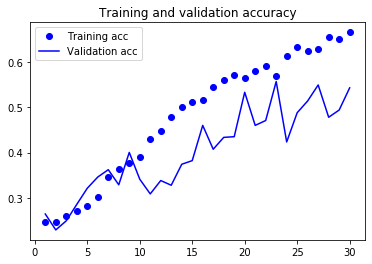
\includegraphics[scale=0.50]{book_model_1_acc}
		\subcaption{\label{subfigure_a}}
	\end{subfigure}
	\begin{subfigure}{0.4\textwidth}
		\centering
		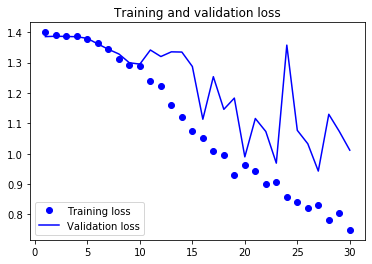
\includegraphics[scale=0.50]{book_model_1_loss}
		\subcaption{\label{subfigure_b}}
	\end{subfigure}
	
	\caption{\label{fig:subcaption_example}Wyniki treningu modelu \protect\subref{subfigure_a} dokładność, \protect\subref{subfigure_b} błąd.}
\end{figure}
\subsection{Strojenie}
Nie wygląda na to, żeby to był dobry kierunek. W sumie to nie wiem jeszcze co należałoby zmienić żeby go dostroić. Na pewno mamy nadpróbkowanie. Może dołożyć BatchNormalisation i więcej Dropoutu?
\subsection{Testowanie}
class0:
Percentage of correctly classified frames: 0.0

class1:
Percentage of correctly classified frames: 100.0

class2:
Percentage of correctly classified frames: 0.0

class3:
Percentage of correctly classified frames: 0.0

Evaluation on test data

125/125 [==============================] - 679s 5s/step

test loss, test acc: [1.3867403992122562, 0.2492963441785771]

\begin{figure}[h]
	\centering
	\begin{subfigure}{0.4\textwidth}
		\centering
		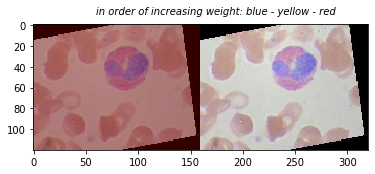
\includegraphics[scale=0.50]{book_model_1_layer_1}
		\subcaption{\label{subfigure_a}}
	\end{subfigure}
	\begin{subfigure}{0.4\textwidth}
		\centering
		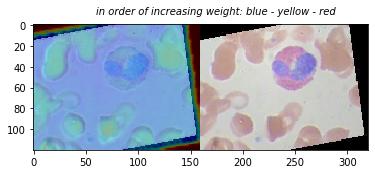
\includegraphics[scale=0.50]{book_model_1_layer_2}
		\subcaption{\label{subfigure_b}}
	\end{subfigure}
	\begin{subfigure}{0.4\textwidth}
		\centering
		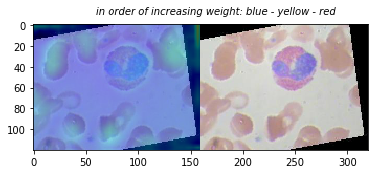
\includegraphics[scale=0.50]{book_model_1_layer_3}
		\subcaption{\label{subfigure_c}}
	\end{subfigure}
	\begin{subfigure}{0.4\textwidth}
		\centering
		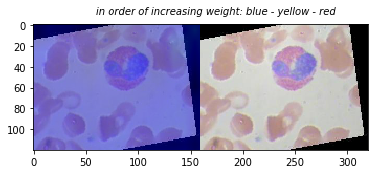
\includegraphics[scale=0.50]{book_model_1_layer_4}
		\subcaption{\label{subfigure_d}}
	\end{subfigure}
	
	\caption{\label{fig:subcaption_example}Obszary aktywacji w kolejnch warstwach \protect\subref{subfigure_a} warstwa 1, \protect\subref{subfigure_b} warstwa 2, \protect\subref{subfigure_c} warstwa 3, \protect\subref{subfigure_d} warstwa 4.}
\end{figure}

\subsection{Wpływ hiperparametrów}
Gdy znajdziesz dobry model tego typu.

\section{MobileNet, pretrenowana sieć konwolucyjna}
\subsection{Struktura}

Jeśli przyjmiemy, że sekwencję warstw: Konwolucyjna, Normalizacja Batcha i ReLu nazywamy A, sekwencję warstw: Depthwise, Normalizacja Batcha i ReLu nazywamy B, zaś sekwencję B,A,B,A nazywamy C, to MobileNet ma strukturę:

\begin{verbatim}
Model: 
_________________________________________________________________
Layer (type)                 Output Shape              Param #   
=================================================================
input_1 (InputLayer)         (None, 120, 160, 3)       0         
conv1_pad (ZeroPadding2D)    (None, 121, 161, 3)       0         
A           
B   
A        
conv_pad_2 (ZeroPadding2D)   (None, 61, 81, 64)        0         
B     
A     
B      
conv_pad_4 (ZeroPadding2D)   (None, 31, 41, 128)       0         
C
conv_pad_6 (ZeroPadding2D)   (None, 16, 21, 256)       0         
C  
C
C
conv_pad_12 (ZeroPadding2D)  (None, 8, 11, 512)        0         
C
flatten_1 (Flatten)          (None, 15360)             0        
dropout_1 (Dropout)          (None, 15360)             0         
dense_1 (Dense)              (None, 256)               3932416   
batch_normalization_1 (Batch (None, 256)               1024      
dense_2 (Dense)              (None, 4)                 1028      
=================================================================
Total params: 7,163,332
Trainable params: 7,140,932
Non-trainable params: 22,400
_________________________________________________________________
\end{verbatim}

\subsection{Trening}

\begin{figure}[h]
	\centering
	\begin{subfigure}{0.4\textwidth}
		\centering
		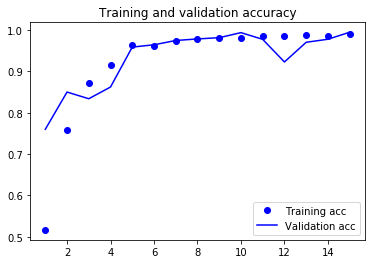
\includegraphics[scale=0.50]{mobileNet_3_acc}
		\subcaption{\label{subfigure_a}}
	\end{subfigure}
	\begin{subfigure}{0.4\textwidth}
		\centering
		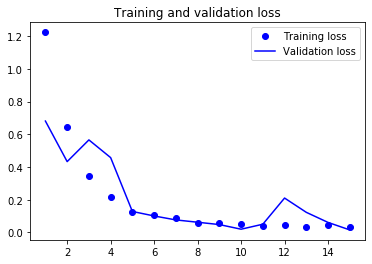
\includegraphics[scale=0.50]{mobileNet_3_loss}
		\subcaption{\label{subfigure_b}}
	\end{subfigure}
	
	\caption{\label{fig:subcaption_example}Wyniki treningu modelu \protect\subref{subfigure_a} dokładność, \protect\subref{subfigure_b} błąd.}
\end{figure}

\subsection{Strojenie}
Model nie wymagał strojenia ani wielokrotnego trenowania, bo przy pierwszym podejściu doszedł do 99\% na zbiorze walidacyjnym oraz funkcja błędu malała wraz ze wzrostem skuteczności.
Parametry:
\begin{verbatim}
frame_size = (120, 160)
activation = 'relu'
output_activation = 'softmax'
optimizer = optimizers.RMSprop(lr=1e-4)#optimizers.Adam(lr = 1e-4)
loss = 'categorical_crossentropy'
metrics = ['acc']
rescale = 1./255
batch_size = 20
epochs=15
validation_set_percentage=80
freezed_layers = range(0) <---- wszystko trainable, bez sensu i pewnie to właśnie 
powód spadku dokładności na nowych danych w porównaniu z treningiem
freeze 21: w 7 epoce 90%/60%
freeze 27: w 7 epoce 95%/50%
freeze 9:  w 7 epoce 93%/57%
Jednak nie, też nie działa, ostatnia kombinacja poniżej:
\end{verbatim}

\begin{figure}[h]
	\centering
	\begin{subfigure}{0.4\textwidth}
		\centering
		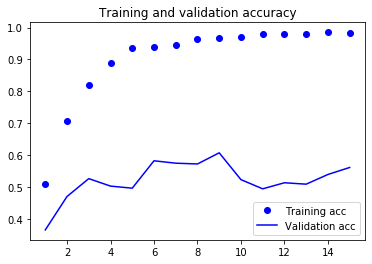
\includegraphics[scale=0.50]{mobileNet_6_acc}
		\subcaption{\label{subfigure_a}}
	\end{subfigure}
	\begin{subfigure}{0.4\textwidth}
		\centering
		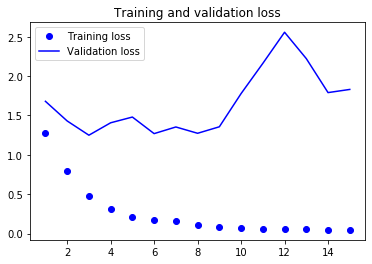
\includegraphics[scale=0.50]{mobileNet_6_loss}
		\subcaption{\label{subfigure_b}}
	\end{subfigure}
	
	\caption{\label{fig:subcaption_example}Wyniki treningu modelu \protect\subref{subfigure_a} dokładność, \protect\subref{subfigure_b} błąd.}
\end{figure}


Zamiast strojenia przetrenowano nowy model (bez zamrożenia warstw). Na przetasowanych danych i ze zmienioną liczbą epok na 10 (żeby uniknąć overfittingu który wystąpił w 12 epoce). Wyniki treningu:

\begin{figure}[h]
	\centering
	\begin{subfigure}{0.4\textwidth}
		\centering
		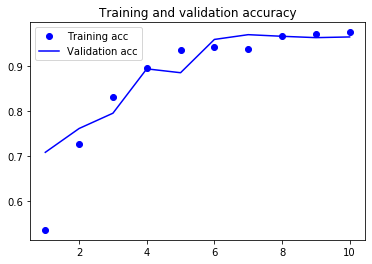
\includegraphics[scale=0.50]{mobileNet_5_acc}
		\subcaption{\label{subfigure_a}}
	\end{subfigure}
	\begin{subfigure}{0.4\textwidth}
		\centering
		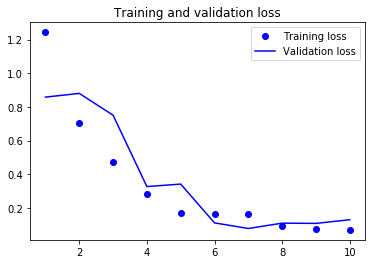
\includegraphics[scale=0.50]{mobileNet_5_loss}
		\subcaption{\label{subfigure_b}}
	\end{subfigure}
	
	\caption{\label{fig:subcaption_example}Wyniki treningu modelu \protect\subref{subfigure_a} dokładność, \protect\subref{subfigure_b} błąd.}
\end{figure}

\subsection{Testowanie}
Dla pierwszej wersji (15 epok):
Gdy wynik predykcji dla danej klasy przekracza 25\% i predykcja jest zgodna z przynależnością do klasy to uznaje się za ramkę dobrze zakwalifikowaną.

class0:
Percentage of correctly classified frames: 18.973214285714285

class1:
Percentage of correctly classified frames: 92.82511210762333

class2:
Percentage of correctly classified frames: 12.584269662921349

class3:
Percentage of correctly classified frames: 12.026726057906458

Dla 10 epok:
class0:
Percentage of correctly classified frames: 23.4375

class1:
Percentage of correctly classified frames: 95.96412556053812

class2:
Percentage of correctly classified frames: 2.0224719101123596

class3:
Percentage of correctly classified frames: 0.6681514476614699
	
\subsection{Wpływ hiperparametrów}
Gdy znajdziesz dobry model tego typu.

\section{Sieć o architekturze U-Net dla segmentacji jednej klasy - to chyba bez sensu}
\subsection{Struktura}
\subsection{Trening}
\subsection{Strojenie}
\subsection{Testowanie}
\subsection{Wpływ hiperparametrów}